\newpage
\subsubsection{Wege zu DevOps}\label{devops_wege}

In der Literatur werden drei Wege bzw. Eckpfeiler für die Einführung erwähnt.
In jedem Fall ist die Verwendung von DevOps eine Investition in Mitarbeiter, Prozesse und Technologien.
\footnote{Kasteleiner/Schwartz, vgl.~\cite{Kasteleiner2019}~[S.211-214]}

Dabei gilt, dass eine solche Einführung niemals als abgeschlossen angesehen werden kann.
\footnote{König/Kugel, vgl.~\cite{Konig2019}~[S.292 - S.293]}
\footnote{Kim et al, vgl.~\cite{Kim2018}}

Diese drei grundsätzlichen Wege von DevOps werden in der Literatur genannt:

\begin{itemize}
    \item \textbf{Flow:}
    Praktiken, um die Zusammenarbeit zwischen den Abteilungen zu verbessern.
    Alles dient dem Ziel die Wertschöpfung für das Unternehmen zu optimieren.

    \item \textbf{Feedback:}
    Um die nächsten Schritte besser bestimmen zu können, sollen die Erfahrungen und Metriken aus dem Betrieb in die Entwicklung zurückfließen.

    \item \textbf{Continuous Learning and Experimentation:}
    Die gesamte Organisation soll die Wertschöpfungskette zum Kunden verstehen und aus den bisherigen Metriken lernen.
\end{itemize}

Um das Experimentieren zu fördern, sollte eine Kultur geschaffen werden in der Fehler toleriert werden.
Dabei sollten Review Prozesse jedoch sicherstellen, dass es durch Fehler zu keinen größeren Ausfällen kommen kann.

Die Einführung von agilen Methoden wie z.B. Scrum einer der ersten Schritte sein, um DevOps zu ermöglichen.
Dies macht Prozesse transparent und erlaubt die Priorisierung von Aufgaben.
\footnote{Kim et al, vgl.~\cite{Kim2018}~[S.16 - S.17]} \\

Der jährlich erscheinende \textsl{State of DevOps Report} von Puppet hat ermittelt, dass die Einführung von DevOps insbesondere für die Produktentwicklung und nicht so sehr für konkrete Projektarbeit geeignet ist.
Das liegt vorallem daran, dass bei Projekten die Anforderungen klarer definiert sind als bei der Entwicklung von Produkten.
\footnote{Wiedemann, vgl.~\cite{Wiedemann2019}~[S.164]}
\footnote{Puppet State of DevOps Report 2020, vgl.~\cite{PUPPET}}

\newpage
\paragraph{Maßnahmen}\label{devops_massnahmen}

Zur Anwendung von DevOps benötigt ein Unternehmen einige technische und organisatorische Maßnahmen.
In der Literatur finden sich hierzu folgende Gemeinsamkeiten:
\footnote{Buchan et. al, vgl.~\cite{Senapathi2018}~[S.2]}
\footnote{Callanan, vgl.~\cite{Callanan2016}~[S.56 - S.57]}
\footnote{Schwarz/Kasteleiner, vgl.~\cite{Kasteleiner2019}~[S.211 - S.214]}

\begin{itemize}
    \item \textbf{Automatisierung:}
    Aufgaben die mehr als zweimal manuell gemacht wurden, sollte automatisiert werden. \footnote{Ozkaya, vgl.~\cite{Ozkaya2019}~[S.3]}

    \item \textbf{Kollaboration und Embedded OPS:}
    Mitarbeiter aus der Betriebsabteilung sollten in die Entwicklungsteams integriert werden.  \footnote{König/Kugel, vgl.~\cite{Konig2019}~[S.294]}

    \item \textbf{Kontinuierliche Entwicklung:}
    Prozesse und Mitarbeiter sollten kontinuierlich weiterentwickelt und optimiert werden.

    \item \textbf{Fokus auf den Kunden:}
    Prozesse und Tätigkeiten sollten stets auf deren Kundennutzen überprüft werden.
    Prozesse, die keinen Wert für den Kunden erzeugen, sollten entfernt werden. \footnote{Ozkaya, vgl.~\cite{Ozkaya2019}~[S.5]} \footnote{Samulat, vgl.~\cite{Samulat2017}~[S.214]}

    \item \textbf{Selbstorganisierte Teams:}
    Kleine selbstorganisierte Teams mit End-to-End-Verantwortung (\textsl{You build it, you run it}). \footnote{Lichtenberger, vgl.~\cite{Lichtenberger2017}~[S.245]}

    \item \textbf{Continuous integration und Testing:}
    Einbindung automatischer Prozesse für Build, Test und Deployment ermöglichen.

    \item \textbf{Continuous Release und Deployment:}
    Durch Automatisierung sollte es einen Weg von Software in die Produktivsysteme geben. \footnote{Buchan et. al, vgl.~\cite{Senapathi2018}~[S.3]}

    \item \textbf{Continuous Monitoring:}
    Infrastruktur und User Verhalten sollten überwacht werden.
    Die Metriken können dann in der Entwicklung berücksichtigt werden.

    \item \textbf{IaC:}
    Infrastruktur sollte replizierbar sein.
    Durch den Einsatz von IaC lässt sich das erreichen.

    \item \textbf{Wiederherstellung:}
    Bei Problemen sollte es einfach möglich sein vorherige Versionen wiederherszustellen, um Ausfälle kurz zu halten.

    \item \textbf{Self Service:}
    Entwickler können selbst die Infrastruktur erstellen, welche sie für ihre Entwicklung benötigen. \footnote{König/Kugel, vgl.~\cite{Konig2019}~[S.293 - S.294]}
\end{itemize}

\paragraph{Migration zu DevOps}

Besonders in Unternehmen, die bereits ohne DevOps Software entwickeln und diese betreiben, lässt sich nicht von jetzt auf gleich eine DevOps Strategie einführen.
Hierzu finden sich in der Literatur folgende mögliche Vorgehensweisen zur nachträglichen Einführung:

Durch Spin-Offs oder Tochterunternehmen können neue Projekte auf der sogenannten \textsl{grünen Wiese} gestartet werden.
Diese werden dann nach und nach in das Unternehmen zurückgeführt. \footnote{Wiedemann, vgl.~\cite{Wiedemann2019}~[S.164]}

Bei einer Umstellung ist es für die Organisation wichtig, einen frühen Erfolg zu erzielen.
Hierzu empfiehlt es sich, kleine inkrementelle Schritte vorzunehmen. \footnote{Kim et al, vgl.~\cite{Kim2018}~[S.58 - S.59]}
% Dabei ist es hilfreich Unterstützung von Nachahmern des Ansatzes zu finden, diese Innovatoren im Unternehmen kann man dan dazu nutzen eine kritische Masse zu erreichen.
% Das Unternehmen Wotif aus Australien hat nach ihrer DevOps Migration ihre Zyklen für das Ausrollen neuer Software von zwei Wochen auf einen Tag verkürzt. \footnote{Callanan, vgl.~\cite{Callanan2016}~[S.56 - S.57]}

\paragraph{DevOps Reifegrade}\label{devops_reifegraden}

Das DevOps Evolution Model wird im jährlichen State Of DevOps Report von Puppet Labs veröffentlicht \footnote{Puppet State of DevOps Report 2020, vgl.~\cite{PUPPET}~[S.10]}
Dort wird der Reifegrad einer DevOps Einführung mittels mehrerer Stufen bewertet:

\begin{figure}[htb]
    \centering
    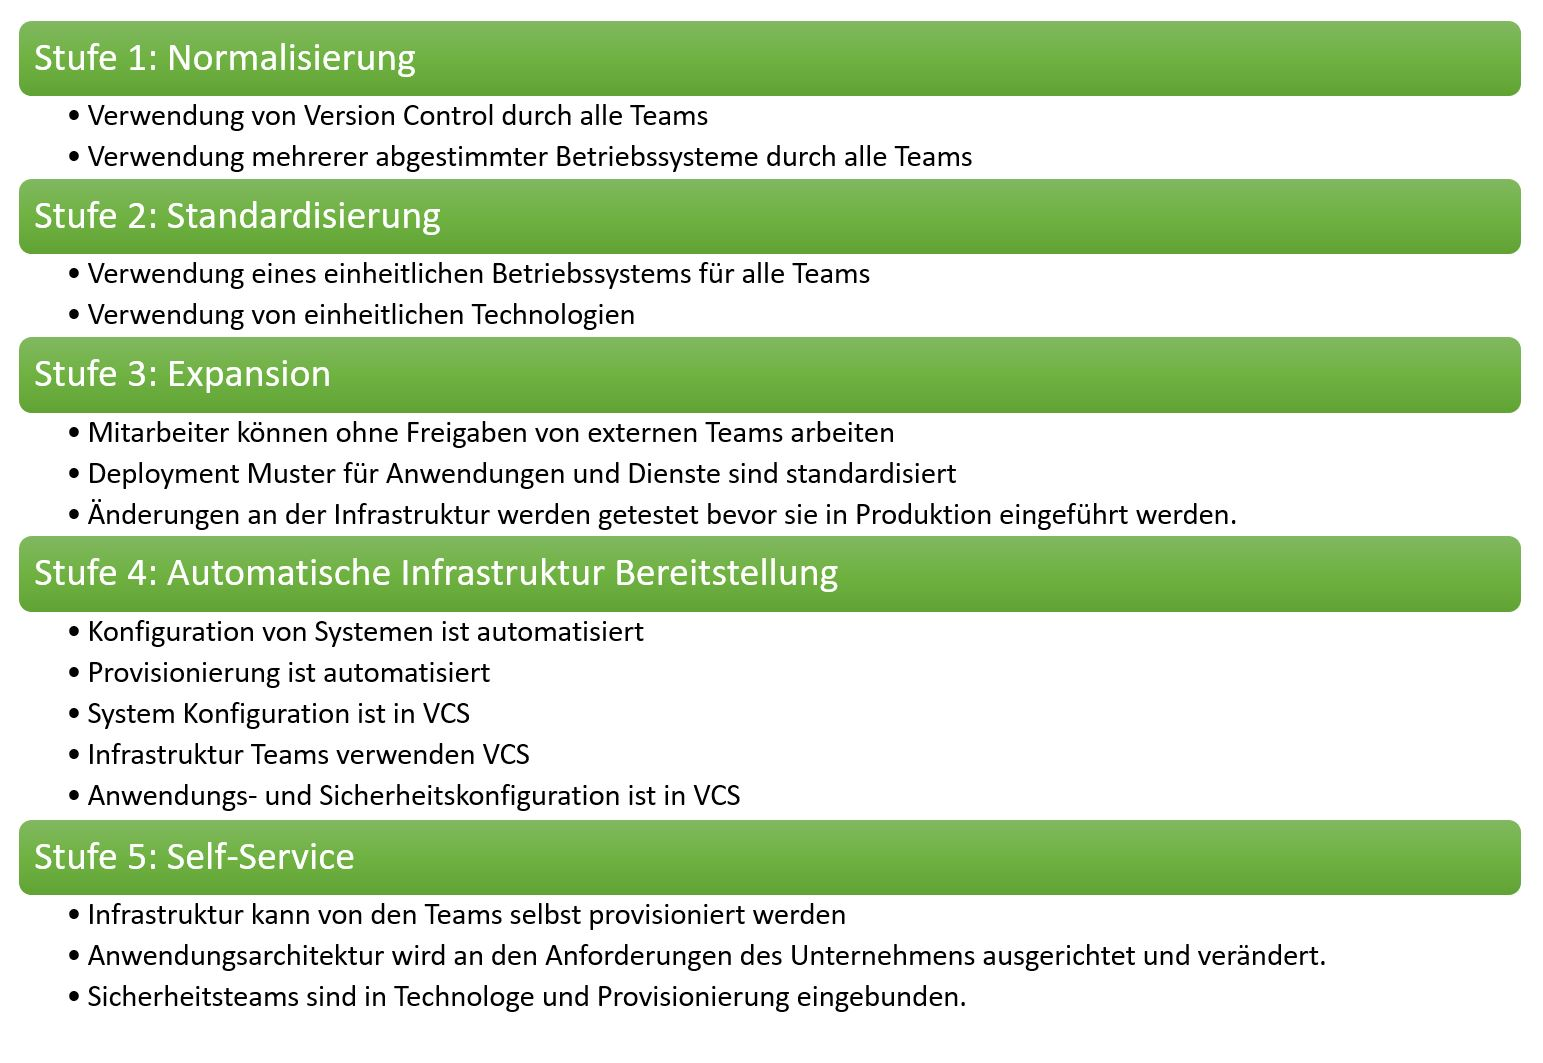
\includegraphics[width=1.0\textwidth]{images/devops_reifegrad.jpg}
    \caption[DevOps Reifegrade]{DevOps Reifegrade}
    \label{fig:DevOps Reifegrade}
\end{figure}

Anhand dieses Models kann ein Unternehmen den eigenen Fortschritt somit überwachen und die weiteren Schritte planen.

%    [RESTE]
%    - A  common  goal  of  all  processes  is  to   eliminate   nonessential   activities   that  consume  resources  away  from  development  and  delivery  of  function-ality  that  provides  quality  to  its  us-ers `(Ozkaya, 5)`
%    - Prozesse auf Kundennutzen prüfen, Kundenwünsche erkennen, nicht werterzeugende Prozesse eliminieren, Trasnsparenz und Qualitätsicherung, Kontiniuierliche Verbesserung `(Samulat, P. 214)`
%    - IT der zwei Geschwindigkeiten (Porter Kurver IT), Economy of Scope vs Scale `(Samulat, P. 207)`
%    - Economy of Scope: Pro Kunde individuell, Einzelfertigung, Individuelle Prozesse
%    - Economy of Scale: Preis/Mengen Strategie, Massenfertigung, Standardprozesse
%    - Mike Gualtieri (2011): "NoOps means application developer will never have to speak to an operations professional again" `(König/Kugel, P. 290)`
%    - Higher levels of DevOps means more self-service offerings for developers, 63% of participants have at least one `(https://puppet.com/resources/report/2020-state-of-devops-report/)`

